
%% !TEX root = manual.tex

\section{Call Graph Visualization}
\label{sec:tutorials:callgraph}
Generating call graphs requires a special build of \sstmacro.

\begin{ShellCmd}
build> ../configure --prefix=$INSTALL_PATH --enable-call-graph
\end{ShellCmd}
The extra flag enables special instrumentation.
In the default build, the instrumentation is not added to avoid overheads.
However, \sstmacro only instruments a select group of the most important functions so the overhead should only be 10-50\%.
After installing the instrumented version of \sstmacro, a call graph must be activated for a given application.

\begin{ViFile}
node {
  app1 {
    call_graph {
      type = call_graph
      output = cachegrind
      group = test
    }
  }
}
\end{ViFile}
After running the above, a \inlineshell{test.callgrind.out} file should appear in the folder based on the group name.
Additionally, a summary CSV file - \inlineshell{test.csv} or other group name - is generated with various aggregate statistics.

To visualize the call graph, you must download KCachegrind: \url{http://kcachegrind.sourceforge.net/html/Download.html}.
KCachegrind is built on the KDE environment, which is simple to build for Linux but can be very tedious for Mac.
The download also includes a QCachegrind subfolder, providing the same functionality built on top of Qt.  
This is highly recommended for Mac users.

\begin{figure}[h]
\centering
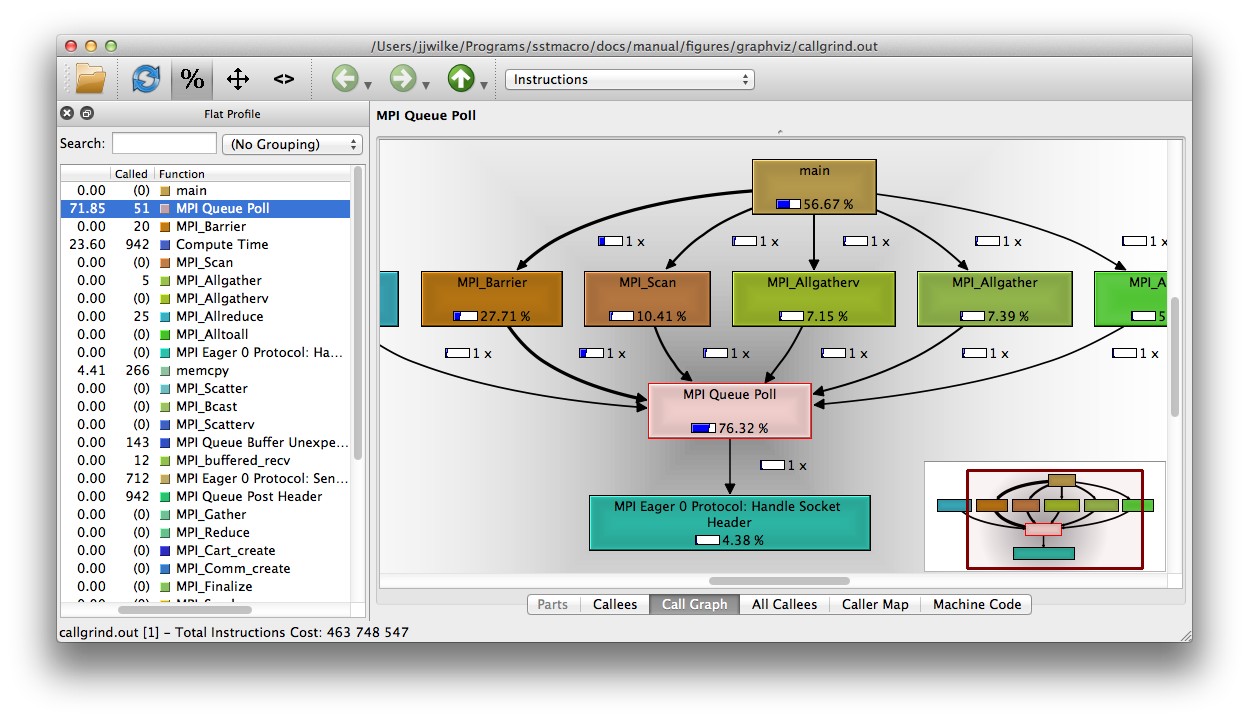
\includegraphics[width=0.95\textwidth]{figures/graphviz/gui.png}
\caption{QCachegrind GUI}
\label{fig:qcgui}
\end{figure}

The basic QCachegrind GUI is shown in Figure \ref{fig:qcgui}.  
On the left, a sidebar contains the list of all functions instrumented with the percent of total execution time spent in the function.
In the center pane, the call graph is shown.  
To navigate the call graph, a small window in the bottom right corner can be used to change the view pane.
Zooming into one region (Figure \ref{fig:qcgraphone}), we see a set of MPI functions (Barrier, Scan, Allgatherv).
Each of the functions enters a polling loop, which dominates the total execution time.  
A small portion of the polling loop calls the ``Handle Socket Header'' function.
Double-clicking this node unrolls more details in the call graph (Figure \ref{fig:qcgraphtwo}).
Here we see the function splits execution time between buffering messages (memcpy) and posting headers (Compute Time).

\begin{figure}[h!]
\centering
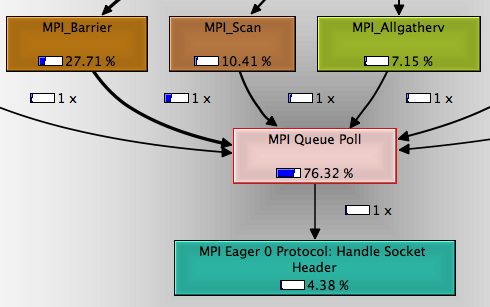
\includegraphics[width=0.55\textwidth]{figures/graphviz/callgraph1.png}
\caption{QCachegrind Call Graph of MPI Functions}
\label{fig:qcgraphone}
\end{figure}

\begin{figure}[h!]
\centering
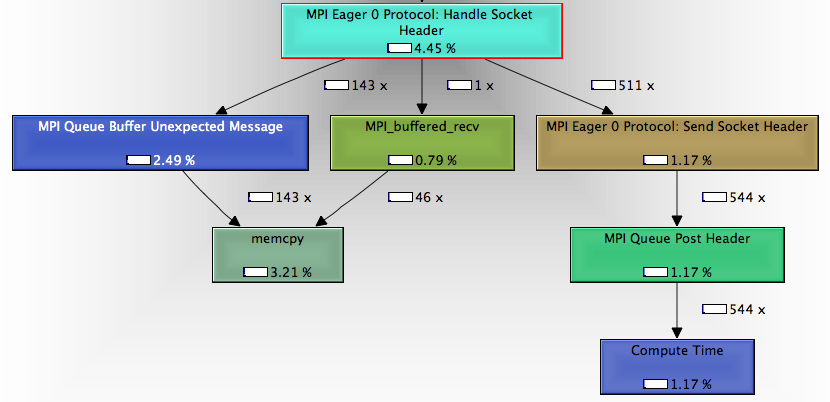
\includegraphics[width=0.75\textwidth]{figures/graphviz/callgraph2.png}
\caption{QCachegrind Expanded Call Graph of Eager 0 Function}
\label{fig:qcgraphtwo}
\end{figure}

In the summary file, each function is broken down into ``self'' time (time spent directly in the function itself)
and time spent in various subroutines.

\begin{ViFile}
app1.rank0.thread0,main,self,40000000000000
app1.rank0.thread0,main,sleep,20000000000000000
app1.rank0.thread0,main,MPI_Init,101362856608
app1.rank0.thread0,main,MPI_Finalize,40013333328
app1.rank0.thread0,main,MPI_Allgather,344587523048
app1.rank0.thread0,main,MPI_Alltoall,80969809408
app1.rank0.thread0,main,MPI_Allreduce,180006666664
app1.rank0.thread0,main,MPI_Barrier,320740095096
app1.rank0.thread0,main,MPI_Gather,160234285648
app1.rank0.thread0,main,MPI_Reduce,161223333064
....
\end{ViFile}
Here is a breakdown of a benchmark for the \inlinecode{main} routine.
A small amount of self-time is shown, along with the time spent in other routines.
Each of these subroutines themselves can also have subroutines:

\begin{ViFile}
app1.rank0.thread0,MPI_Allgather,self,121499999400
app1.rank0.thread0,MPI_Allgather,memcopy,3034190336
\end{ViFile}

